\documentclass[10pt,a4paper,twocolumn,twoside]{article}
\usepackage[utf8]{inputenc}
\usepackage[catalan]{babel}
\usepackage{multicol}
\usepackage{graphicx}
\usepackage{adjustbox}

\usepackage{hyperref}

\usepackage{fancyhdr}
\usepackage{times}
\usepackage{titlesec}
\usepackage{multirow}
\usepackage{lettrine}
\usepackage[top=2cm, bottom=1.5cm, left=2cm, right=2cm]{geometry}
\usepackage[figurename=Fig.,tablename=TAULA]{caption}
\usepackage{verbatim}
\usepackage{float}
\usepackage{ulem}
\usepackage{pdfpages}
\usepackage[hyphenbreaks]{breakurl}
\usepackage[caption=false]{subfig}
\usepackage{caption}
\captionsetup[table]{position=bottom}

\usepackage[toc,page]{appendix}

\captionsetup[table]{textfont=sc}
\usepackage{titlesec}

\setcounter{secnumdepth}{4}

\titleformat{\paragraph}
{\normalfont\normalsize\bfseries}{\theparagraph}{1em}{}
\titlespacing*{\paragraph}
{0pt}{3.25ex plus 1ex minus .2ex}{1.5ex plus .2ex}

\makeatletter
%same as \subsubsection but level 4
\renewcommand\subparagraph{\@startsection{subparagraph}{5}{\z@}%
                                     {-3.25ex\@plus -1ex \@minus -.2ex}%
                                     {1.5ex \@plus .2ex}%
                                     {\normalfont\normalsize\bfseries}}
% number \paragraph
\setcounter{secnumdepth}{5}

\makeatother

\author{\LARGE\sffamily Gerard Martínez Espelleta}
\title{\Huge{\sffamily Visualització, creació i millora de terrenys 3D}}
\date{\today}

\newcommand\blfootnote[1]{%
  \begingroup
  \renewcommand\thefootnote{}\footnote{#1}%
  \addtocounter{footnote}{-1}%
  \endgroup
}

%
%\large\bfseries\sffamily
\titleformat{\section}
{\large\sffamily\scshape\bfseries}
{\textbf{\thesection}}{1em}{}

\setlength\parindent{0pt}
\begin{document}

\fancyhead[LO]{\scriptsize Gerard Martínez Espelleta: Visualització, creació i millora de terrenys 3D}
\fancyhead[RO]{\thepage}
\fancyhead[LE]{\thepage}
\fancyhead[RE]{\scriptsize EE/UAB TFG INFORMÀTICA: Visualització, creació i millora de terrenys 3D}

\fancyfoot[CO,CE]{}

\fancypagestyle{primerapagina}
{
   \fancyhf{}
   \fancyhead[L]{\scriptsize TFG EN ENGINYERIA INFORMÀTICA, ESCOLA D'ENGINYERIA (EE), UNIVERSITAT AUTÒNOMA DE BARCELONA (UAB)}
   \fancyfoot[C]{\scriptsize \today , Escola d'Enginyeria (UAB)}
}

%\lhead{\thepage}
%\chead{}
%\rhead{\tiny EE/UAB TFG INFORMÀTICA: TÍTOL (ABREUJAT SI ÉS MOLT LLARG)}
%\lhead{ EE/UAB \thepage}
%\lfoot{}
%\cfoot{\tiny{February 2015, Escola d'Enginyeria (UAB)}}
%\rfoot{}
\renewcommand{\headrulewidth}{0pt}
\renewcommand{\footrulewidth}{0pt}
\pagestyle{fancy}

%\thispagestyle{myheadings}
\twocolumn[\begin{@twocolumnfalse}

%\vspace*{-1cm}{\scriptsize TFG EN ENGINYERIA INFORMÀTICA, ESCOLA D'ENGINYERIA (EE), UNIVERSITAT AUTÒNOMA DE BARCELONA (UAB)}

\maketitle

\thispagestyle{primerapagina}
%\twocolumn[\begin{@twocolumnfalse}
%\maketitle
%\begin{abstract}
\begin{center}
\parbox{0.915\textwidth}
{\sffamily
\textbf{Resum--}
Durant les últimes dècades, la visió de mapes tridimensionals ha avançat moltíssim des de l'aparició de Google Maps l'any 2005, el qual va popularitzar i fer disponible al públic general aquest servei. No obstant les noves tecnologies com la visualització tridimensional del relleu només s'apliquen a zones molt poblades deixant de banda una gran part de la superfície del territori.\\
En aquest treball farem ús de tècniques de Deep Learning per a crear una xarxa neuronal que ens permeti aplicar superresolució a un seguit d'imatges del terreny, a les que posteriorment afegirem un relleu i mostrarem en un entorn 3D pel qual ens podrem desplaçar amb la intenció de poder explorar tot el territori català.
\\
\\
\textbf{Paraules clau-- }Visor 3D, Deep Learning, GAN, Generative Adversative Network, Mapa, Superresolució, Web\\
\\
%\end{abstract}
%\bigskip
%\begin{abstract}
\bigskip
\\
\textbf{Abstract--} 
Over the last few decades, three-dimensional map viewing has come a long way since the advent of Google Maps in 2005, which made this service popular and available to the general public. However, new technologies such as three-dimensional relief visualization are only applied to heavily populated areas, leaving apart a large part of the territory's surface. \\
In this work we will use Deep Learning techniques to create a neural network that allows us to apply superresolution to a series of terrain images, to which we will later add a relief and show in a 3D environment through which we can move with the intention to be able to explore the entire catalan territory.
\\
\\
\textbf{Keywords-- } 3D Visor, Deep Learning, GAN, Generative Adversative Network, Map, Superresolution, Web\\
}

\bigskip

{\vrule depth 0pt height 0.5pt width 4cm\hspace{7.5pt}%
\raisebox{-3.5pt}{\fontfamily{pzd}\fontencoding{U}\fontseries{m}\fontshape{n}\fontsize{11}{12}\selectfont\char70}%
\hspace{7.5pt}\vrule depth 0pt height 0.5pt width 4cm\relax}

\end{center}

\bigskip
%\end{abstract}
\end{@twocolumnfalse}]

\section{Introducció - Context del treball}

Un dels avantatges del que disposem avui en dia en comparació amb fa uns anys és la possibilitat d'utilitzar mapes en línia per situar-nos, obtenir indicacions, o simplement investigar el terreny. De fet, des de l'aparició del primer servidor de mapes en línia ("Xerox PARC Map Viewer") l'any 1993, aquest servei ha anat millorant any rere any, passant per visors de mapes de renom com "Terraserver" \ l'any 1998 o ``Nasa World Wind'' l'any 2003. No obstant això, no va ser fins a l'any 2005 que es va popularitzar aquest tipus de servei amb l'aparició de Google Maps, el qual es va tornar el principal servidor de mapes en línia del mercat.\\
\blfootnote{$\bullet$ E-mail de contacte: 1531236@uab.cat}
\blfootnote{$\bullet$ Menció realitzada: Computació}
\blfootnote{$\bullet$ Treball tutoritzat per:Felipe Lumbreras Ruiz (Departament de Ciències de la Computació)}
\blfootnote{$\bullet$ Curs 2021/22}
\hfill \break

Avui en dia, aquests serveis han anat evolucionant, permetent aplicar diferents capes a la vista com imatges satèl·lit, de relleu, del trànsit o fins i tot en els últims anys permetent la visualització del relleu sobre imatges satèl·lit en 3D o l'opció de poder visualitzar a vista de carrer la majoria del globus.

Així i tot, visors com el de \textit{Google Earth} o \textit{Apple Maps} només ofereixen una bona representació del terreny en zones que les companyies consideren més interessants. És a dir, en zones d'alta afluència de persones, com podrien ser grans ciutats o zones universitàries. Si sortim d'aquests límits, les imatges es comencen a veure borroses i sense relleu visible.

En aquest projecte es farà us de tècniques de processat d'imatges i de Deep Learning per a crear un model que sigui capaç d'augmentar significativament la resolució d'una imatge. A part es crearà un visor tridimensional accessible de manera online que serà capaç de mostrar tot el mapa de Catalunya mitjançant crides a un servidor, d'on anirà descarregant les imatges (que seràn arreglades pel nostre model) i els valors del relleu per posteriorment ajuntar-les en un objecte tridimensional i col·locar-lo en un punt de l'espai, creant així un mapa.

\subsection{Objectius}
L'objectiu principal d'aquest treball és el de crear una aplicació que ens permeti, a partir d'un conjunt d'imatges satèl·lit, millorar notablement la resolució d'aquestes mitjançant xarxes neuronals que apliquin tècniques de superresolució i posteriorment afegir-hi un relleu creant així un objecte tridimensional. Finalment, crearem un entorn tridimensional pel qual ens puguem desplaçar en el que es trobin tots aquests objectes anteriorment creats.\\

És a dir, crear un mapa d'alta resolució i amb relleu pel qual puguem navegar i on sigui possible veure tot el territori català. Per tal de definir millor el projecte, l'hem dividit en els següents propòsits.\\

Aquests serien:
\begin{enumerate}
\item \textbf{Obtenció d'imatges satèl·lit: }La resolució d'aquest objectiu consistirà en investigar diverses fonts d'on es puguin obtenir les imatges satèl·lit necessàries per mostrar el territori. Un cop les tinguem crearem un script per poder-les obtenir fàcilment.

\item \textbf{Obtenir els valors del relleu: }Aquests són necessaris per crear els models tridimensionals. Per poder completar aquest objectiu s'haurà de trobar una font que ens ofereixi valors del relleu català i posteriorment crear un script que ens permeti obtenir-los.

\item \textbf{Creació d'una xarxa que ens permeti fer superresolució: }Millorar la qualitat de les imatges mostrades a la nostra aplicació passant aquestes per una xarxa neuronal que apliqui un algoritme de superresolució. Investigar els tipus de xarxa que permeten aplicar l'algoritme anteriorment mencionat, i un cop escollit el model de xarxa a realitzar s'haurà d'escollir un entorn per dissenyar-la i entrenar-la.

\item \textbf{Creació d'una xarxa que ens permet millorar el relleu obtingut: }Obtenir el relleu més realista que sigui possible, passant el relleu descarregat de la font escollida per una xarxa neuronal que el millori. Buscar el tipus de xarxa més adient per dur a terme aquest tipus de feina, i un cop escollit, dissenyar i entrenar en el mateix entorn que en el punt anterior o en un altre diferent.

\item \textbf{Crear entorn 3D: }Crear un aplicatiu que permeti agafar una imatge del relleu i una imatge satèl·lit i ajuntar-les en un objecte tridimensional que es mostrarà en un entorn pel qual ens podrem moure.
\end{enumerate}

%\begin{figure*}[H]
%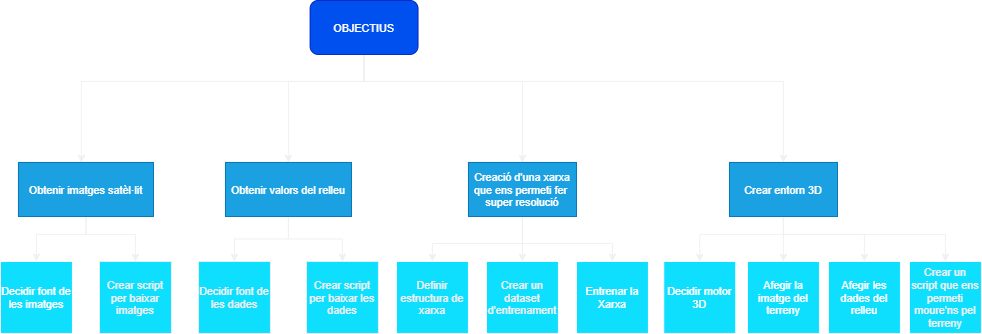
\includegraphics[scale = 0.5]{img/Objectius.png}
%\end{figure*}

\subsection{Metodologia}
Per tal de dur a terme aquest projecte d'una manera ordenada i rigorosa es farà ús de la metodologia de \textit{Kanban} \cite{kanban}.
Aquesta metodologia és considerada una metodologia \textit{"agile"} que ens obliga a portar un control precís del que s'ha fet, el que s'està fent i el que queda per fer mitjançant la repartició de la feina en tres columnes diferents que representen aquests estats.\\

Per tal de poder aplicar-la, es farà ús d'una eina anomenada \textit{Trello} \cite{trello} i es crearan tres columnes: una pels objectius complerts, una pels objectius en els quals estem treballant i una última pels objectius que encara no s'han fet.\\

Afegidament, es programaran un conjunt de reunions amb el tutor per poder fer un correcte seguiment i comprovar que tots els resultats es van assolint degudament.

\subsection{Planificació}

Per explicar la planificació del treball i alhora, per ajudar a l'organització d'aquest, s'ha realitzat un diagrama de Gantt organitzat per setmanes, el qual es pot trobar al dossier.
Aquest permet obtenir una vista general dels objectius programats, de manera que resulta molt senzill saber quines feines s'han de fer, quant temps s'ha de dedicar a cada tasca i, per tant, quan ha d'estar acabada cada una d'elles.\\

%\begin{figure}[H]
%\centering
%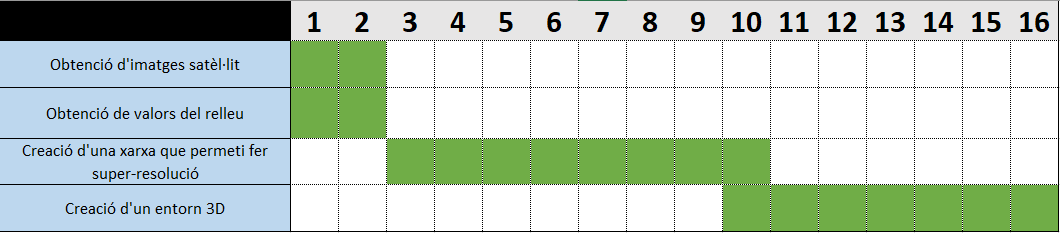
\includegraphics[width=.5\textwidth]{img/diagramaSetmana.png}
%\caption{Diagrama de Gantt}
%\end{figure}

Els apartats als quals dediquem més temps són aquells referents a la creació de xarxes neuronals, ja que a part del disseny, s'haurà de dedicar temps a entrenar-les i testejar-les. A més també s'haurà de dedicar una quantitat considerable de temps al visor 3D, ja que es destinarà molt temps a revisar la documentació de l'eina seleccionada.\\
Al dossier, es podrà trobar informació més detallada sobre com s'ha distribuït el temps de cada subobjectiu.

\section{Estat de l'art}
Aquest projecte compta amb dues parts importants. La primera és la generació d'imatges satèl·lit d'alta resolució a partir d'imatges de baixa resolució, i la segona part és la generació de terrenys tridimensional a partir de les imatges prèviament creades.\\

A continuació es mostrarà l'estat de l'art amb relació als algoritmes i a les tecnologies existents.

\subsection{Algoritmes existents de superresolució}
La superresolució és una tècnica molt important en el món de la visió per computador i s'utilitza principalment en el món mèdic o en el món de la vigilància. Aquesta consisteix en, a partir d'una imatge amb soroll o molt pixelada, millorar la seva resolució, ja sigui suavitzant-la, editant els valors dels píxels o fins i tot afegint-n'hi de nous.\\

Una de les estructures de xarxa més usada és la \textit{UNet}. Aquesta és una xarxa neuronal del tipus convolucional i es fa servir principalment per la segmentació d'imatges, és a dir, per poder diferenciar diferents elements dins d'una sola imatge.
No obstant això, també pot ser usada per realitzar superresolució d'imatges modificant una mica la seva arquitectura, com es pot observar en els casos següents:

\subsubsection{RUNet}
Es tracta d'una implantació d'una UNet, però afegint-hi sumes després de cada "block" de la xarxa, creant així una estructura de \textit{residual blocks} \cite{RUNet}. Aquestes sumes permeten a la xarxa aprendre estructures més complexes.
\begin{comment}
\begin{figure}[H]
\centering
\includegraphics[width=.5\textwidth]{img/RUNet.png}
\caption{Estructura d'una RUNet \\(font:https://github.com/cerniello/Super\_Resolution\_DNN)}
\end{figure}
\end{comment}
\subsubsection{Dense-UNet }
La Dense-UNet \cite{DenseUNet} combina les característiques de la UNet i de la Dense-Net. És a dir que cada block no només rep informació del block anterior sinó de tots els blocks que l'han precedit. Això ajuda a combatre la pèrdua d'informació causada per les capes de "downsampling" que incorpora la UNet.
\begin{figure}[h]
\centering
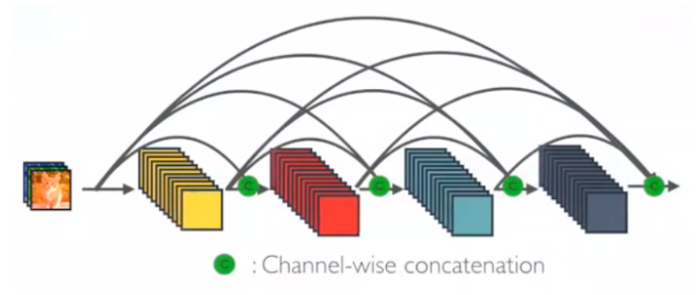
\includegraphics[width=.5\textwidth]{img/dense.png}
\caption{Estructura d'una connexió densa\\ (font:https://towardsdatascience.com/review-densenet-image-classification-b6631a8ef803)}
\end{figure}

\subsubsection{SRGAN}
Una altra estructura de xarxa molt utilitzada en aquest context i que ha anat guanyant popularitat durant els últims anys és la de les xarxes adversàries generatives, també conegudes com a GAN.\\
Aquesta estructura consta de dues xarxes:
\begin{itemize}
\item\textbf{Una xarxa generativa }encarregada de generar les imatges en superresolució
\item\textbf{Una xarxa discriminativa }encarregada de valorar si la imatge creada per la xarxa anterior és correcta o no.
\end{itemize}
Aquestes dues xarxes competeixen l'una contra l'altra de manera que només pot guanyar una de les dues (el guany d'una és el ``loss'' de l'altra). D'aquesta manera la xarxa no s'entrena per millorar contra ella mateixa, sinó que ho fa amb la intenció d'enganyar al discriminador. És per això que els resultats són molt sovint capaços d'enganyar fins i tot a un humà.\\

La \textbf{SRGAN} \cite{SRGAN} és un tipus de GAN utilitzada per a millorar la resolució d'imatges. Aquesta agafa una imatge en baixa resolució i mitjançant l'agregació de nous píxels, intenta millorar la qualitat d'aquesta.
\begin{figure}[h]
\centering
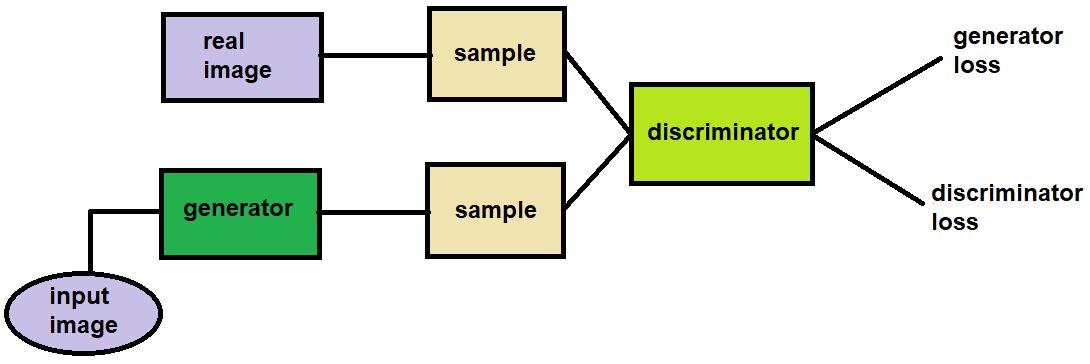
\includegraphics[width=.5\textwidth]{img/GAN.png}
\caption{Estructura d'una GAN}
\end{figure}

\subsection{Visors de relleu existents}
Per altra banda, a l'hora de realitzar el visor 3D, hem pogut observar que també existeixen entorns que realitzen les funcions que nosaltres volem desenvolupar, tot i que tenen les limitacions anteriorment mencionades en la introducció.
\subsubsection{Google Maps}
Google Maps és un servei web de visió de mapes oferit per Google que ofereix imatge per satèl·lit, visió aèria, visió de carrer, imatges 360º, indicacions per viatjar juntament amb l'estat del trànsit i horaris de transport públic i fins i tot imatges dels interiors d'alguns edificis. És usada per més d'un bilió de persones d'arreu del món cada més i ha estat desenvolupada en javascript i crides AJAX (la part del client)
\subsubsection{Google Earth}
Google Earth és un altre servei de visió de mapes que superposa les imatges i el relleu sobre un globus terraqüi, oferint així una sensació més realista. Aquesta plataforma té imatges del 98\% del globus terraqüi, a més de contenir dos globus més; un de la Lluna i l'altre de Mart. També compta amb un visor d'estrelles i un simulador de vol que et permet volar per terreny realista i ubicacions reals. A part, també inclou guies que et permeten visitar llocs turístics o monuments sense sortir de casa.
\begin{figure}[h]
\centering
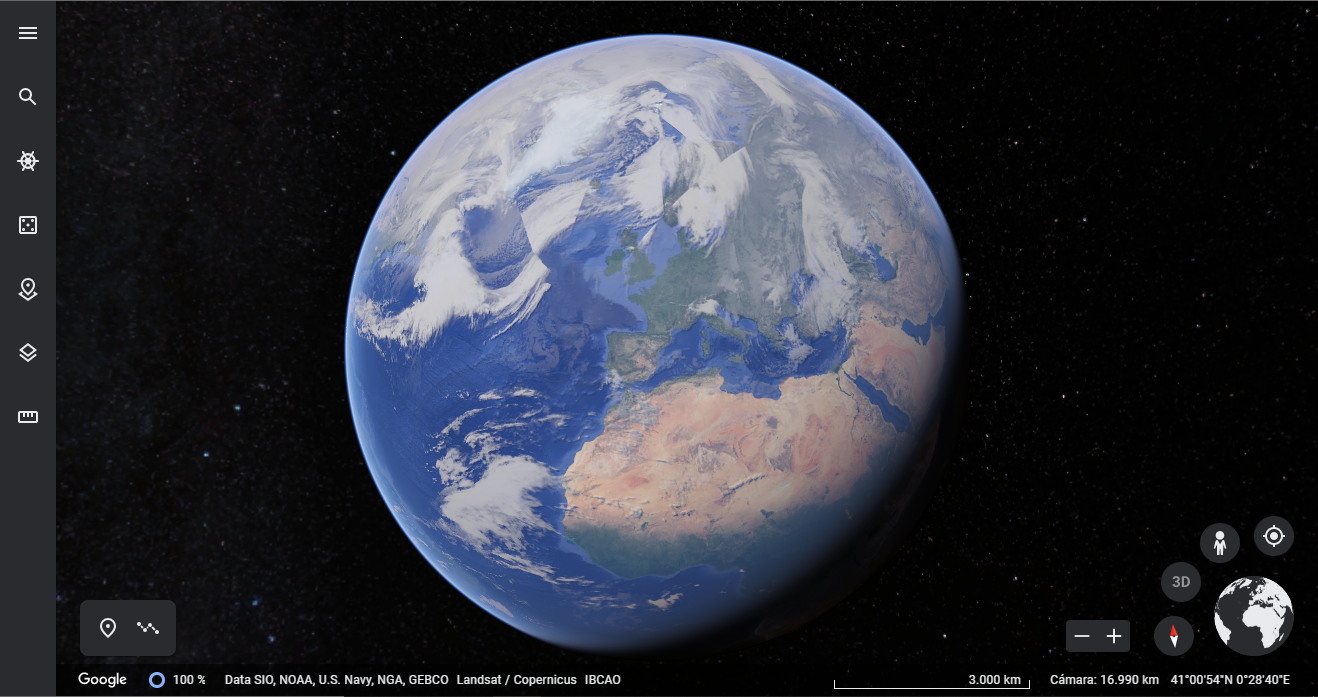
\includegraphics[width=.5\textwidth]{img/googleEarth.png}
\caption{Visor de mapes Google Earth}
\end{figure}
\begin{comment}
\subsubsection{Apple Maps}
Apple Maps és un visor de mapes creat per Apple per a ser usat en els seus dispositius, tot i que també pot ser usat a través del motor de cerca \textit{DuckDuckGo} el qual l'utilitza com a servei de mapes. Aquest visor, a part de mostrar mapes amb el seu relleu, inclou eines que ofereixen indicacions a l'hora de desplaçar-se.
\end{comment}
\subsubsection{Unity}
Unity és un motor de videojoc multiplataforma creat per Unity Technologies. Està disponible com a plataforma de desenvolupament per a Microsoft Windows, OS X, Linux. La plataforma de desenvolupament té suport de compilació amb diferents tipus de plataformes com per exemple Android, Windows, Linux o aplicacions web.
\subsubsection{Unreal Engine}
Unreal Engine és un motor de videojoc d'ordinador i consoles creats per l'empresa Epic Games. Està escrit en C++, la qual cosa permet un alt grau de portabilitat i ofereix diverses eines addicionals de gran ajuda per a dissenyadors i artistes. Afegidament, també té suport de compilació per a diferents plataformes igual que l'entorn anteriorment mencionat.
\subsubsection{Godot}
Godot Engine és un motor gràfic de desenvolupament de videojocs, multiplataforma, gratuït i de codi obert, distribuït sota la llicència MIT. Permet desenvolupar videojocs en 2D i en 3D mitjançant un sistema jeràrquic de nodes i escenes, i inclou les eines necessàries per al desenvolupament de manera centralitzada i visual, seguint la mateixa línia que altres motors gràfics com Unity o Unreal Engine.
\subsubsection{Three.js}
Three.js és una biblioteca escrita en JavaScript per a crear i mostrar gràfics animats en 3D en un navegador web i pot ser usada en conjunció amb elements HTML5, SVG o WebGL. El codi font és lliure i està emmagatzemat en un repositori de GitHub.\\

A continuació podem veure una taula comparativa dels diferents entorns de desenvolupament anteriorment mencionats:

\begin{table}[H]
\caption{Comparació dels diferents entorns}
\begin{adjustbox}{width=\columnwidth,center}
\begin{tabular}{|ll|c|c|c|c|}
\hline
\multicolumn{2}{|r|}{\textit{\textbf{Motor}}}          & \multicolumn{1}{l|}{\multirow{2}{*}{\textbf{Unity}}} & \multicolumn{1}{l|}{\multirow{2}{*}{\textbf{Unreal Engine}}} & \multicolumn{1}{l|}{\multirow{2}{*}{\textbf{Godot}}} & \multicolumn{1}{l|}{\multirow{2}{*}{\textbf{Three js}}} \\ \cline{1-2}
\multicolumn{2}{|l|}{\textit{\textbf{Característica}}} & \multicolumn{1}{l|}{}                                & \multicolumn{1}{l|}{}                                        & \multicolumn{1}{l|}{}                                & \multicolumn{1}{l|}{}                                   \\ \hline
\multicolumn{2}{|l|}{\textbf{Codi obert}}              & No                                                   & Si                                                           & Si                                                   & Si                                                      \\ \hline
\multicolumn{2}{|l|}{\textbf{Llenguatge}}              & C\#                                                  & C++                                                          & C\#                                                  & Javascript                                              \\ \hline
\multicolumn{2}{|l|}{\textbf{Visor}}                   & Aplicació                                            & Aplicació                                                    & Aplicació                                            & Navegador                                               \\ \hline
\end{tabular}
\end{adjustbox}
\end{table}
\section{Desenvolupament del treball}


\subsection{Obtenció de dades}
El primer pas per tal de dur a terme el projecte és una bona elecció de la font que utilitzarem per aconseguir les imatges. És necessari trobar una font que no només ens ofereixi imatges satèl·lit, sinó d'on també es puguin aconseguir dades del relleu i imatges amb una major qualitat per poder entrenar correctament la xarxa de superresolució. Un cop feta la recerca, s'han trobat les següents fonts d'on és possible descarregar les dades requerides:

\subsubsection{Sentinel2}
Sentinel2 \cite{Sentinel} és una missió d'observació del grup \textit{Copérnico}. Aquesta compta amb dos satèl·lits que permeten la captura d'imatges multiespectrals (de 13 bandes), d'infrarojos i de l'espectre electromagnètic. Afegidament, compta amb una API bastant senzilla d'utilitzar i que ofereix resultats amb un molt baix temps de resposta. Malgrat això, s'ha decidit no fer ús dels serveis que ens ofereix Sentinel, ja que l'API que s'utilitza per demanar les imatges és de pagament i es prefereix buscar alguna plataforma gratuïta.

\subsubsection{NASA}
La NASA \cite{NASA} és l'agència d'exploració espacial dels Estats Units, i permet fer ús de la seva API de \textit{web map service} d'una manera gratuïta amb un simple registre. Tot i que amb aquesta API es poden obtenir imatges de tot el globus i de forma gratuïta, es pot notar com les imatges rebudes són d'una qualitat considerablement menor que les que es podien obtenir amb el satèl·lit Sentinel. A més, és bastant casual que aquestes continguin núvols que evitin que es pugui veure la superfície correctament. Finalment, es va descartar aquesta font perquè a part de tenir imatges de no massa bona qualitat, el temps de resposta era superior a 10 segons, la qual cosa perjudicaria l'experiència de l'usuari que utilitzés el visor 3d.

\subsubsection{Google Earth}
Google Earth \cite{Earth} es un visor en línia de mapes en 3d. La seva API permet obtenir dades del relleu d'un punt només indicant-hi les coordenades. Aquesta API és gratuïta i fàcilment accessible mitjançant un compte de Google. Tanmateix, aquesta plataforma va ser descartada quan es va decidir que es faria ús de mapes d'altura per calcular el relleu.

\subsubsection{IGN}
L'Institut Nacional de Geografia \cite{ign}, és una entitat pública encarregada d'investigar i organitzar les dades geogràfiques del país. Aquest compta amb una API gratuïta que permet obtenir imatges satèl·lit d'una manera ràpida i senzilla.
Tot i això, no s'ha fet ús d'aquesta API, ja que no oferia dades sobre el relleu del territori.

\subsubsection{ICGC}
L'Institut Cartogràfic i Geològic de Catalunya \cite{icgc} és també una entitat pública encarregada d'investigar i emmagatzemar dades geogràfiques, però en aquest cas, dades exclusivament del territori català. Aquesta API també ofereix l'opció de descarregar mapes d'altures on es veu fàcilment el relleu del terreny o imatges de major qualitat capturades des d'un avió.
En el cas de les imatges satèl·lit, aquestes són imatges obtingudes de Sentinel2 i arreglades per la mateixa organització per eliminar núvols i millorar-ne la qualitat. És per aquesta sèrie de motius que s'ha decidit fer ús d'aquesta font d'imatges pel projecte.\\

Un cop escollida la font (i ja que la nostra aplicació necessita moltes imatges per funcionar de manera correcta), s'ha creat un script que permet descarregar-les de manera automàtica només passant-li les coordenades desitjades.\\

Aquest està escrit amb python i compta amb dues funcions principals:
\begin{enumerate}
\item{\textbf{Convertidor de sistema de coordenades}}: L'API de ICGC fa ús d'un sistema de coordenades anomenat \textit{'EPSG:25831'}, mentre que normalment en aplicacions com Google Maps es fa ús d'un altre sistema anomenat \textit{'EPSG:4326'}. Per tant, per poder introduir les coordenades desitjades d'una manera més còmoda, aquesta funció converteix les dades d'un sistema a l'altre.
\item{\textbf{Obtenció de les imatges}}: Un cop obtingudes les coordenades en el sistema desitjat, només s'ha de realitzar la sol·licitud d'imatge al servidor i emmagatzemar la resposta d'aquest en cas que no retorni un error.
\end{enumerate}
A part també es va crear un script de revisió de dataset, el qual comprovava que les imatges descarregades fossin adequades (mitjançant tècniques com el percentatge de píxels negres o el tamany de la imatge) i en cas que no ho fossin les eliminava.

\subsection{Creació d'algoritmes de superresolució}

Per tal de poder dur a terme aquest treball, s'han construït i entrenat dos models diferents de xarxa neuronal: una UNet i una GAN. Amb la intenció de complir aquest objectiu, s'ha fet ús de diferents llibreries de python que ens facilitaven el treball.\\Les més destacades són:
\begin{itemize}
\item\textbf{opencv: }És una llibreria de codi obert que ofereix un gran conjunt d'eines orientades a la visió per computador. En el nostre cas va ser útil a l'hora de llegir les imatges i passar-les a la xarxa, ja que abans d'entregar-les s'havien de modificar els canals d'aquestes.
\item\textbf{pytorch: }És un entorn dissenyat per a python que permet el disseny, creació i entrenament de xarxes neuronals, així com la seva posterior avaluació. Ha sigut la llibreria base a partir de la qual s'han creat ambdues xarxes.
\item\textbf{numpy: }És una llibreria matemàtica compilada en C++ i dissenyada per a python que ens permet realitzar operacions a una gran velocitat. Ha sigut important a l'hora de realitzar certs càlculs i obtenir els resultats de la xarxa

\end{itemize}

\subsubsection{Creació d'una UNet}
Com s'ha mencionat anteriorment, s'ha triat crear una UNet degut principalment a la seva senzillesa; com que és una xarxa totalment convolucional, el tamany de la imatge que sigui introduïda, serà exactament igual que el tamany de la imatge que retorni la xarxa. A més, s'ha pensat que permetria suavitzar els contorns dels píxels en les imatges pixelades de manera que quedarien més suaus, donant un efecte de millor resolució.
\paragraph{Creació d'un dataset per a la UNet}
Una xarxa neuronal necessita moltes imatges per poder ser entrenada i que doni uns resultats acceptables. És per això que es va decidir crear un Dataset propi amb imatges d'alta resolució i de baixa. Per aconseguir això es van utilitzar dos scripts; un primer que es baixava imatges d'alta qualitat de Catalunya i un altre que "netejava" aquest dataset, eliminant així imatges en negre (fora de la zona del territori) o arxius d'errors.\\

Un cop executats els dos arxius, es va aconseguir un dataset amb més de 70.000 imatges en alta resolució. El següent pas va ser disminuir la resolució d'aquestes per simular l'input esperat. Això es va realitzar d'una manera senzilla aprofitant l'algoritme de redimensionament d'imatges que utilitza la llibreria \textbf{opencv}. Aquesta feia ús de nearest neighbourg com a mètode de selecció de valor de píxel a l'hora de fer una redimensió, per tant, només es va haver de disminuir la mida de les imatges i després augmentar-la per poder obtenir una imatge pixelada i amb una baixa qualitat.

\paragraph{Disseny de la xarxa}
La xarxa consta de tres parts, una part de codificació, una part intermitja i una part de descodificació. Cada una d'aquestes parts està formada per una estructura a la qual anomenarem \textit{Block}. Cada \textit{Block} està format per dues convolucions i dues funcions d'activació de tipus \textit{ReLU} agrupades de la següent manera:
\begin{figure}[H]
\centering
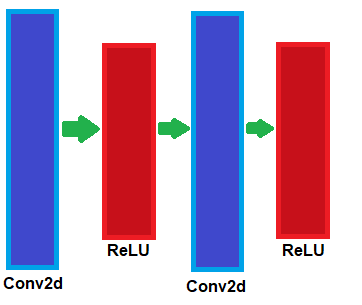
\includegraphics[width=0.3\textwidth]{img/graficaBlock.png}
\caption{Estructura d'un Block de la UNet}
\end{figure}

\textbf{A la part de codificació} l'objectiu de la xarxa és extreure el major nombre de característiques que li sigui possible de la imatge. Per aconseguir aquest objectiu anirà unint una sèrie de \textit{blocks} amb operacions de \textit{max pooling} de 2x2. Això farà que alhora que el nombre de característiques augmenta, el tamany de la imatge va reduint-se. En el cas d'aquest treball, la part de codificació compta amb 4 \textit{blocks} de profunditat.\\

\textbf{La part intermitja} només comptarà amb un \textit{block}, el qual augmentarà un cop més les característiques i passarà les dades a la part de descodificació.\\

\textbf{La part de descodificació}, amb el mateix tamany que la de codificació és l'encarregada de generar la imatge que retorna la xarxa. En aquest cas, els \textit{blocks} estaran units amb convolucions verticals, o el que és el mateix operacions de convolució transposades. Aquesta operació permetrà reduir el nombre de característiques, tornant la imatge a la seva mida original. Afegidament, cada \textit{block} que formi aquesta descodificació, rebrà també les característiques que hem extret a la fase de codificació per poder formar una imatge final satisfactòria.

%\subsection{Creació de la xarxa de millora del relleu}

\subsubsection{Creació d'una GAN}
Un cop valorats els resultats obtinguts amb la UNet visibles a l'apartat \textit{\nameref{section:resUNet}} es va observar que per intentar aconseguir uns millors resultats es podia fer ús d'una \textit{Generative Adversative Network} o \textit{GAN}.\\

Una GAN \cite{GAN} és un model de xarxa neuronal capaç de generar un conjunt de dades de sortida amb les mateixes qualitats que el conjunt de dades d'entrada. Aquesta consisteix en dues xarxes neuronals que competeixen l'una contra l'altra de manera que només pot guanyar una de les dues (el \textit{gain} d'una és el \textit{loss} de l'altra.\\

La mecànica principal d'aquest tipus de xarxa és la de l'entrenament "indirecte" mitjançant un discriminador (una altra xarxa capaç d'identificar si un \textit{input} s'assembla al resultat esperat), de manera que la xarxa no s'entrena per treure una imatge en concret, sinó que s'entrena per a enganyar al discriminador.\\
\paragraph{Creació d'un dataset per a la GAN}
Per tal d'entrenar aquesta xarxa, es va crear un dataset similar al creat per a la UNet amb imatges en alta resolució i en baixa resolució. Així i tot, les imatges de sortida d'aquesta xarxa tenen un tamany diferent de les imatges d'entrada.\\ És per aquest motiu, que es va crear un dataset format per un conjunt d'imatges de 120x120 píxels, les quals serien les imatges entrants i un altre grup d'imatges de 240x240 píxels, les quals representarien la sortida òptima de la xarxa.\\

Aquestes es van obtenir a partir d'una redimensió de les imatges del dataset original. D'aquesta manera es podia donar per segur que eren exactament de la mateixa àrea.
\paragraph{Disseny de la xarxa}
Tal com s'ha comentat una GAN consta de dues parts, un discriminador i un generador:

\subparagraph{Discriminador}
És l'encarregat de decidir si la imatge que se li passa com a input és una imatge en alta definició o no. Està format per:\\

\textbf{Una convolució d'entrada seguida per una Leaky ReLu: }Mitjançant aquestes capes iniciem l'extracció de característiques de la imatge.\\

\textbf{Una sèrie de blocks: }Els quals extreuen les característiques de la imatge. Cada block està format per una convolució, un batch normalitzation (que normalitza les dades de sortida de la convolució) i una funció d'activació Leaky ReLU, tal i com podem observar a la figura inferior.
\begin{figure}[h]
\centering
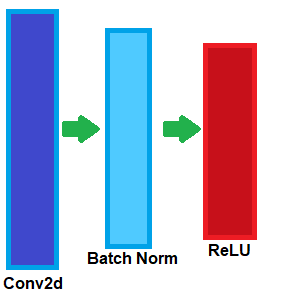
\includegraphics[width=0.25\textwidth]{img/blockdiscriminator.png}
\caption{Estructura d'un Block del Discriminador}
\end{figure}
\textbf{Dues funcions Lineals: }Aquestes són les encarregades de convertir totes les característiques extretes de la imatge a un sol valor que definirà si la imatge entrant és en alta definició o no.\\

\textbf{Una funció sigmoid: }Aquesta funció d'activació ens permet col·locar el valor obtingut de les funcions lineals dins de l'interval [0,1]. D'aquesta manera aquesta funció retornarà la probabilitat de que la imatge sigui en alta resolució o no.
\subparagraph{Generador}
És la xarxa encarregada de generar imatges que siguin capaces d'enganyar al discriminador.\\
Aquesta està formada per:\\

\textbf{Una convolució inicial seguida d'una funció ReLU: }Utilitzada per extreure les característiques inicials de la imatge.\\

\textbf{Una estructura mitjana:} La qual consisteix en un número de residual Blocks seguit d'una convolució, un batch normalitzation i una suma de la x inicial amb la x resultant al final de l'estructura. (Fig\ref{mitjana})

\begin{figure}[h]
\centering
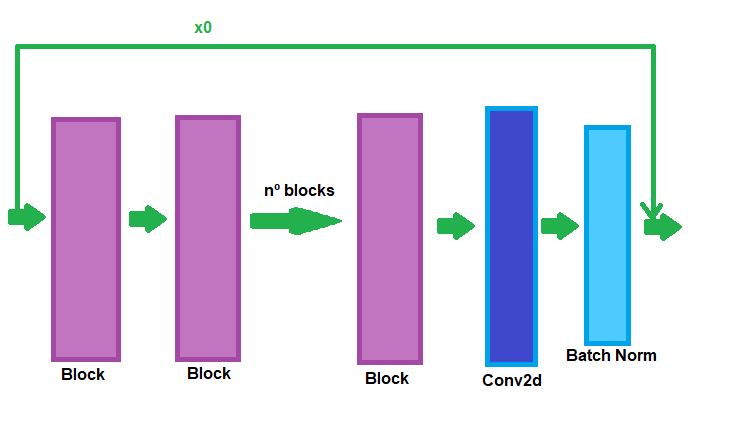
\includegraphics[width=0.5\textwidth]{img/partdelmitg.png}
\caption{Estructura mitjana}
\label{mitjana}
\end{figure}
\begin{comment}
A la figura \ref{img:block} es mostra l'estructura d'un dels blocks residuals mencionats anteriorment. Podem notar com també es fa la suma de característiques al final de cada un d'ells.

\begin{figure}[h]
\centering
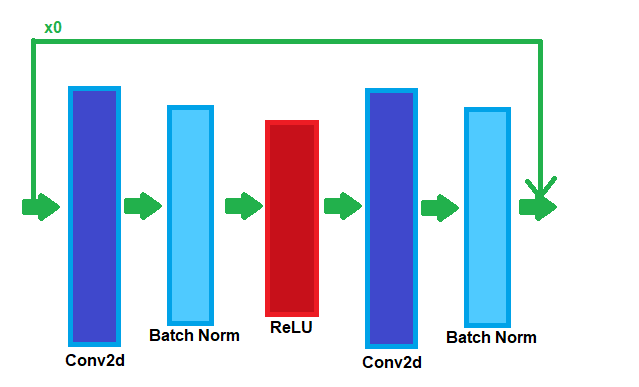
\includegraphics[width=0.5\textwidth]{img/blockgenerator.png}
\caption{Estructura d'un Block del Generator}
\label{img:block}
\end{figure}
\end{comment}
\textbf{Una estructura final d'upsampling: }Aquesta estructura consta d'una convolució, un pixel shuffle (el qual reordena els píxels permetent així una convolució per subpíxels) i una ReLU final. (Fig\ref{ultimblock})\\

\begin{figure}[h]
\centering
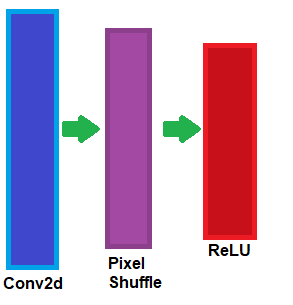
\includegraphics[width=0.25\textwidth]{img/finalBlockGen.png}
\caption{Estructura de l'últim block del Generador}
\label{ultimblock}
\end{figure}

\textbf{Una última convolució: }Permet tornar a obtenir 3 canals de sortida (RGB) com la imatge original.
\\
\subsection{Creació de l'entorn 3D}
Per tal de poder fer visibles els resultats obtinguts en els anteriors apartats, s'ha de comptar amb un entorn tridimensional on no només puguem veure les imatges del terreny, sinó també la representació del seu relleu. Per tal d'aconseguir això, s'ha discutit entre els diferents motors gràfics que s'han pogut veure a l'estat de l'art.\\

Tot i que tots eren molt complets i que els que eren motors de videojocs, ja tenien incloses llibreries per a realitzar el càlcul de físiques i renderitzats, s'ha optat per a triar \textit{Three.js} com a llibreria per al nostre entorn, ja que, a part de ser una llibreria de codi obert, en ser la seva interfície una aplicació en línia ofereix una major integració amb la resta de components que ja han sigut creats en altres llenguatges, a part de permetre un accés a l'eina molt més senzill i lliure d'instal·lacions per part de l'usuari final.

\subsubsection{Three.js}
Three.js és una llibreria de JavaScript que permet crear i mostrar gràfics i animacions en 3D en un navegador Web.\\

Per tal que aquest motor funcioni, s'ha de crear un arxiu HTML que tingui importada la llibreria de Three.js i tots els arxius que continguin el codi. En el cas de la nostra aplicació, hem creat sis arxius JavaScript que ajuden a portar el control de tota la simulació:\\
\paragraph{scene.js}
Es tracta de l'arxiu principal del projecte, en aquest es carregarà l'escena, juntament amb la càmera, l'skybox i el bucle de l'animació, el qual és el bucle principal del motor. Des d'aquí es realitzaran les crides a tots els altres arxius.

\paragraph{checkload.js}
Aquest arxiu conté les funcions que seran usades per \textit{scene.js} per comprovar si el terreny que està a punt de trepitjar l'usuari està carregat o no. En cas que no estigui carregat, es farà una crida al servidor per obtenir les imatges del terreny i dibuixar-les. Aquest últim pas el farem mitjançant una eina de JavaScript anomenada \textit{promises}. Aquesta ens permet executar una funció sense esperar al seu resultat i, un cop s'aconsegueixi el resultat, utilitzar-lo. D'aquesta manera la càrrega de terreny no aturarà el bucle principal de la pàgina sinó que es durà a terme en segon pla.

\paragraph{terrain.js}
Aquest arxiu és l'encarregat de dibuixar el terreny en pantalla. Compta amb dues funcions principals:
\begin{itemize}
\item \textbf{LoadTerrain:} A aquesta funció se li passa una imatge (una de les imatges inicials) i el seu relleu i ho dibuixa per pantalla a la posició que se li indiqui.
\item \textbf{LoadTerrainBinary:} Aquesta funció rep el valor de la imatge retornada pel servidor quan li fem una crida des de l'arxiu \textbf{checkload.js}. Un cop rebuda, la descodifica (ja que la imatge ve en hexadecimal) i torna a fer una crida al servidor per a obtenir el seu relleu. Un cop aconseguit el relleu, el descodifica i extreu els seus valors per posteriorment afegir-los a la imatge i dibuixar el terreny com un pla tridimensional a la posició que se li indica.
\end{itemize}
Tal com hem comentat ambdues funcions anteriors operen amb una imatge del relleu i amb una del terreny.

\begin{figure}[H]
\centering
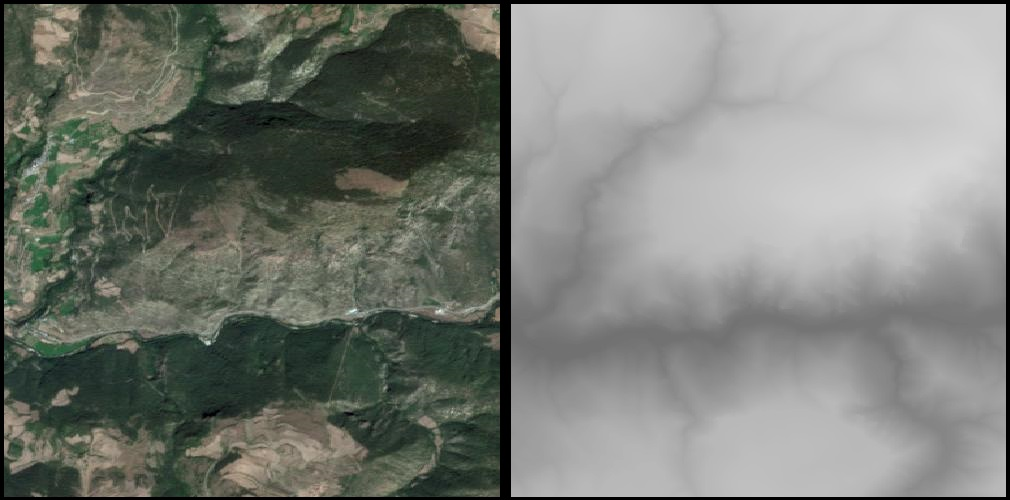
\includegraphics[width=0.45\textwidth]{img/img_relleu.png}
\caption{Imatge del terreny i imatge del relleu}
\end{figure}

Per tal d'extreure el relleu de la imatge fem ús d'una funció la qual analitza el valor de cada píxel de la nostra imatge de relleu i l'emmagatzema en una llista. Posteriorment recorre els valors dels vèrtexs del nostre pla on tenim la imatge satèl·lit i va assignant els valors de les altures d'aquests a partir de les dades emmagatzemades a la llista.

\begin{figure}[h]
\centering
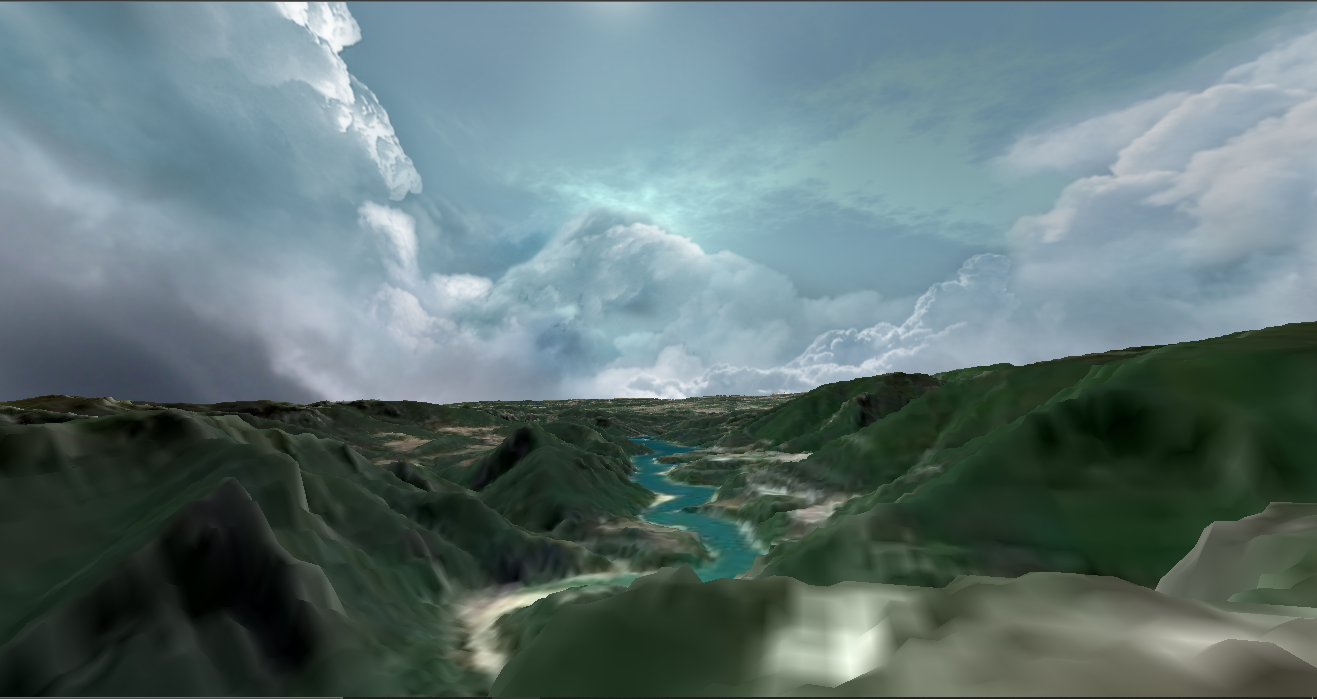
\includegraphics[width=0.45\textwidth]{img/relleu.png}
\caption{Exemple de terreny amb el relleu generat}
\end{figure}

\paragraph{memorysaver.js}
Aquest arxiu és l'encarregat de gestionar que el nostre visor 3D no ocupi més memòria de la necessària, ja que si fos així aquest es tornaria lent i complicat de fer servir.\\Això ho aconsegueix mitjançant una funció que és cridada cada cop que es genera terreny nou.\\

Aquesta comprova si les caselles que s'han generat anteriorment es troben encara dintre del rang de visió de l'usuari, i en cas que no sigui així les elimina i actualitza les variables de posició.
\paragraph{automate.js}
És l'arxiu encarregat de carregar les imatges inicials automàticament. Aquest compta amb una funció que carrega un cert nombre d'imatges (passat com a paràmetre), així com el seu relleu i ho afegeix en pantalla automàticament.

\paragraph{interface.js}
Aquest fitxer controla el que es visualitza a la interfície web. Aquest compta amb tres estats:\\
\textbf{Un estat inicial}\\
En aquest estat l'usuari acaba d'entrar a la pàgina i, per tant, encara s'han de carregar els components i les imatges inicials. Per evitar que aquest s'hagi de quedar esperant davant d'una pantalla negra, es mostra una pantalla de càrrega en la qual es mostra el nom de la web, així com una icona i un símbol de càrrega.
\begin{figure}[H]
\centering
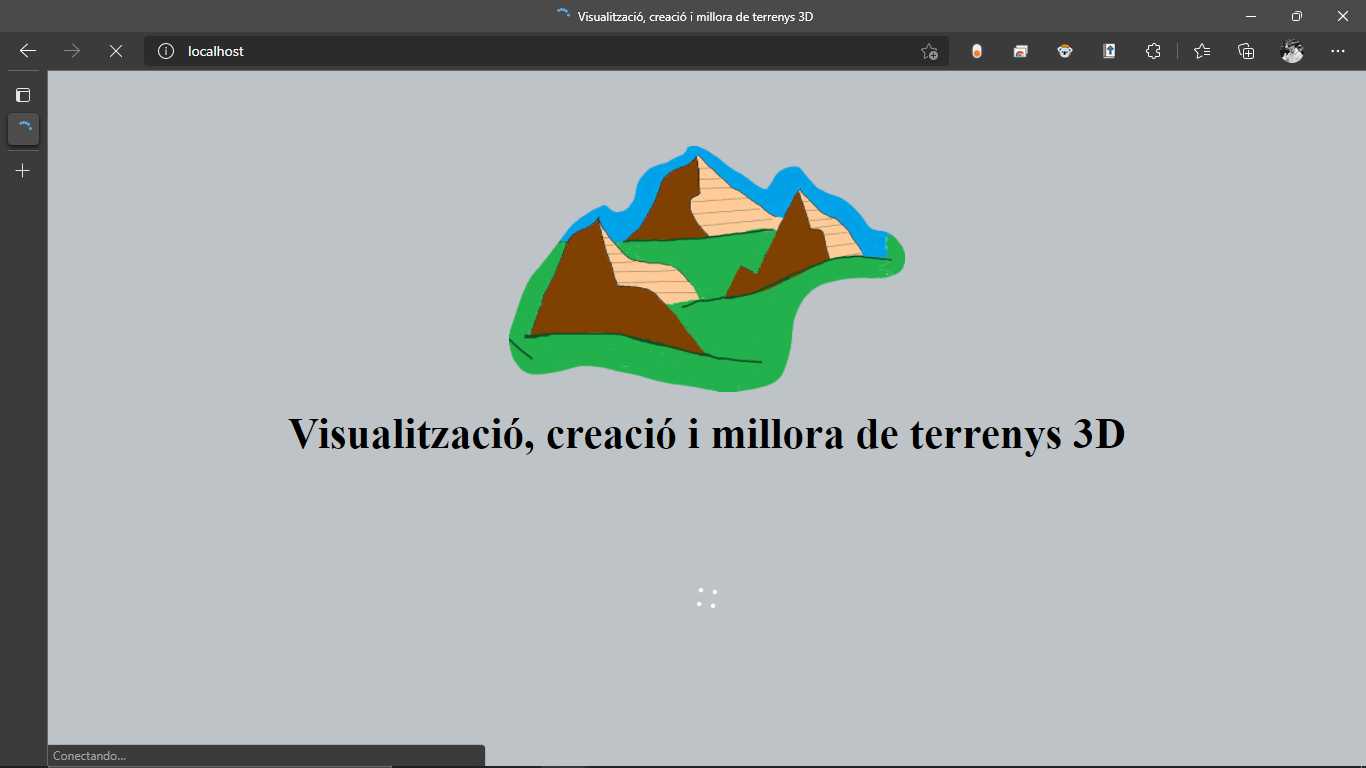
\includegraphics[width=0.45\textwidth]{img/loadingScreen.png}
\caption{Pantalla de càrrega}
\end{figure}
Aquesta pantalla es mantindrà fins que totes les imatges inicials hagin sigut processades i es comencin a afegir a l'escena.\\

\textbf{Un segon estat}\\
Un cop el relleu ha estat carregat i visible per pantalla, aquest arxiu mostrarà a l'usuari la vista d'aquest relleu, però hi superposarà una finestra amb les instruccions per desplaçar-se per la pàgina.
\begin{figure}[h]
\centering
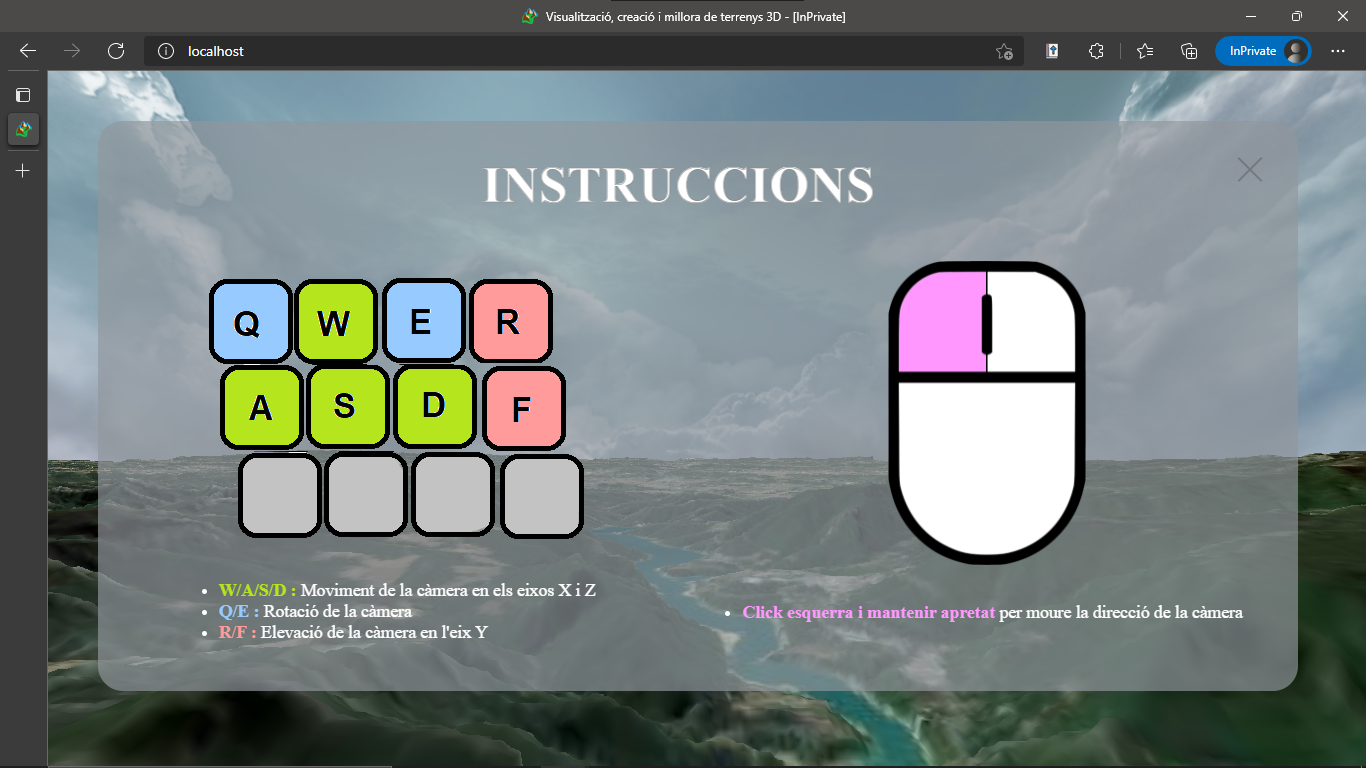
\includegraphics[width=0.45\textwidth]{img/instruccions.png}
\caption{Instruccions superposades a la vista del relleu}
\end{figure}
Un cop l'usuari les hagi llegit, podrà prémer la creu que es troba a la cantonada superior dreta de la finestra. En pressionar-la, passarem al \textbf{tercer estat}, on desapareixerà la finestra i l'usuari ja es podrà moure lliurement per l'entorn.

\begin{figure*}[t]
\centering
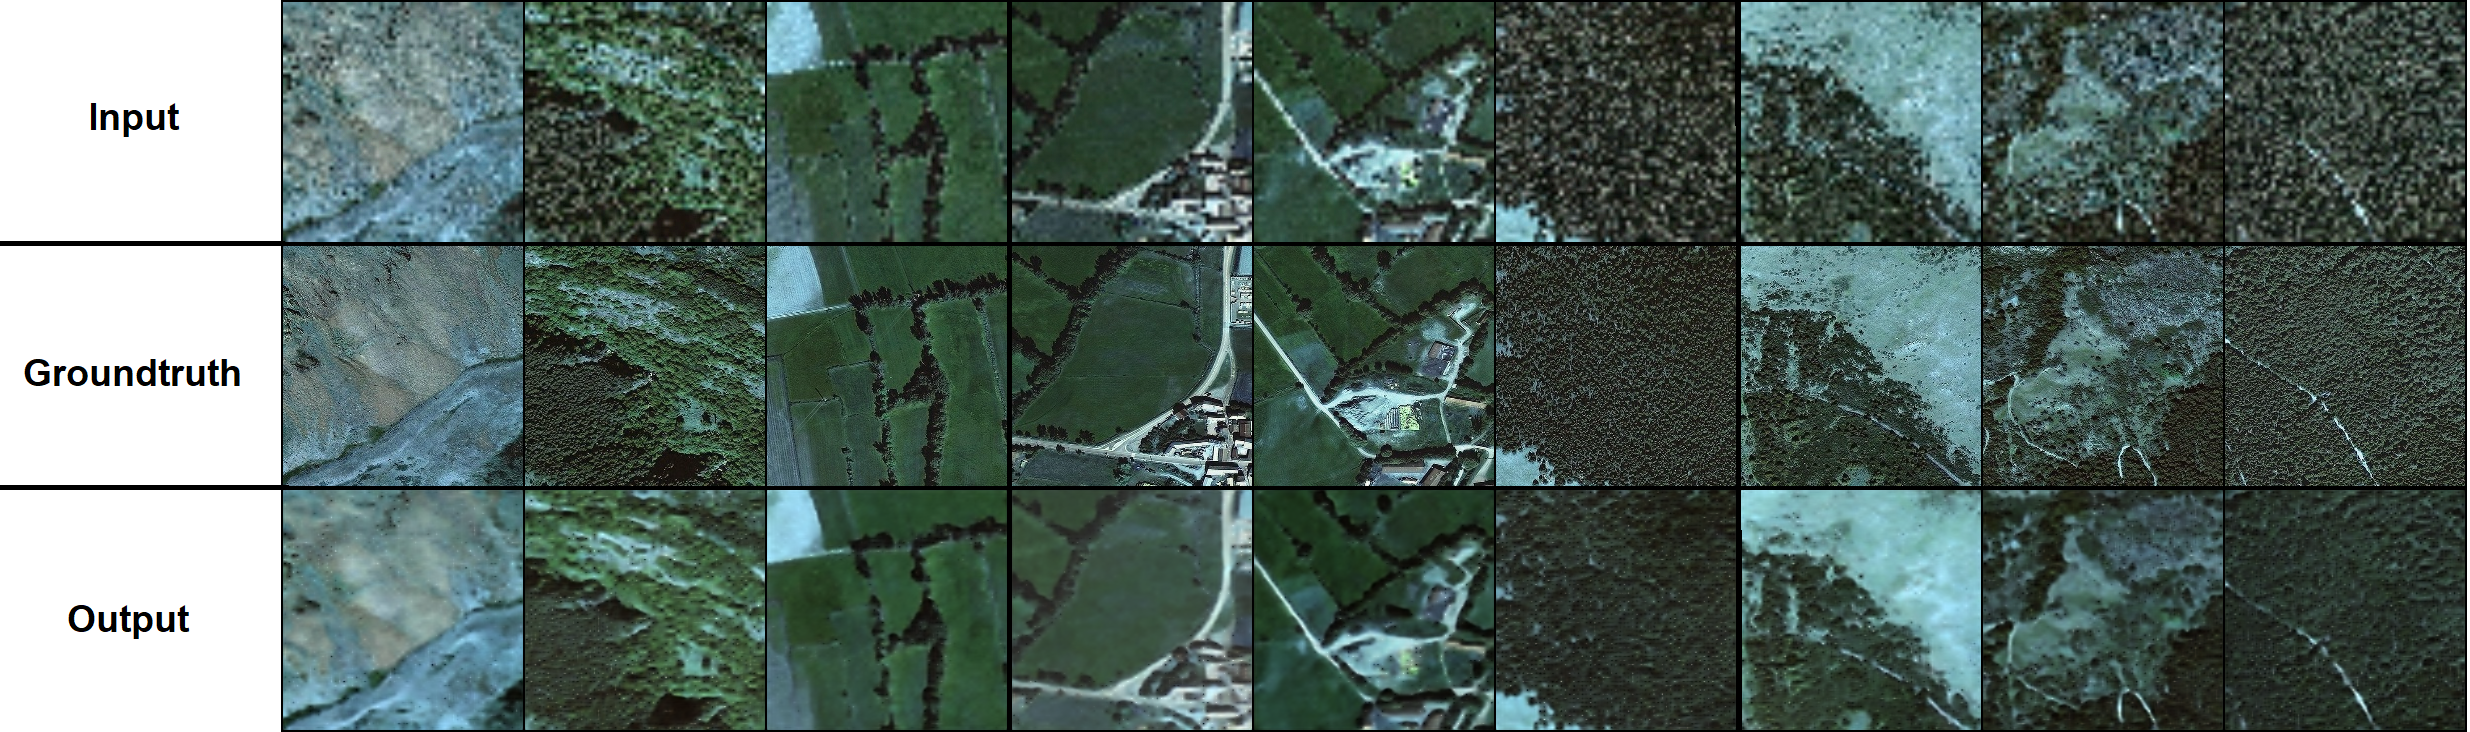
\includegraphics[width=1\textwidth]{img/comparacio.png}
\caption{Resultats obtinguts amb la UNet}
\label{fig:resultsUNet}
\end{figure*}
\subsubsection{Estructura física de l'entorn}

Per poder rebre les dades tractades, l'aplicació web necessita connectar amb un servidor per tal que aquest faci les operacions necessàries. Per aquest motiu, s'ha creat la següent estructura:
\begin{figure}[h]
\centering
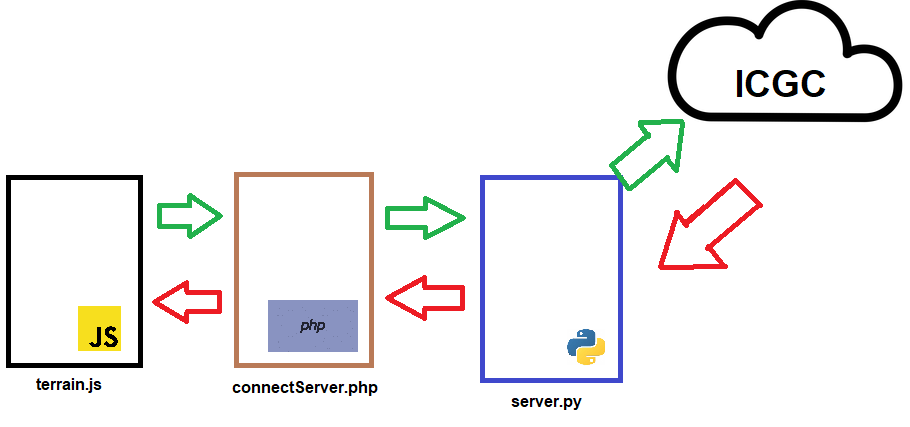
\includegraphics[width=0.3\textwidth]{img/disseny.png}
\caption{Estructura física de l'entorn}
\label{img:fisica}
\end{figure}
Tal com podem veure a la figura \ref{img:fisica}, quan l'arxiu de càrrega de terreny noti que necessita dades noves, contactarà amb l'arxiu \textit{connectServer.php} mitjançant una crida asíncrona d'\textit{AJAX}. Quan aquest rebi la crida amb les dades necessàries per obtenir les imatges, es connectarà al servidor \textit{server.py} mitjançat l'ús de sockets, i aquest, un cop rebi la connexió, demanarà les imatges mitjançant un \textit{HTTPRequest} al servidor del \textbf{ICGC}. Un cop hagi obtingut les imatges, les tractarà si així s'escau i les retornarà a l'arxiu \textit{PHP} mitjançant sockets, el qual respondrà la crida \textit{AJAX} retornant les dades de la imatge desitjada en hexadecimal al nostre arxiu de càrrega de terreny, el qual haurà de descodificar la imatge per poder-la afegir com a textura al nostre relleu.

\subsubsection{Processament de les dades}
Quan al servidor li arriba una ordre de càrrega d'imatge, a aquest se li indica si cal processar-la o no. En cas positiu, un cop ha obtingut la imatge del servidor del \textbf{ICGC}, la descodifica i la divideix en 36 subimatges. A continuació carrega la xarxa neuronal prèviament entrenada i aplica el tractament de les imatges passant-les per la xarxa. Un cop acabat el procés les imatges són novament ajuntades i enviades a l'arxiu \textit{.php} mitjançant sockets tal com s'ha explicat en l'apartat anterior.
%%%%%%%%%%%%%%%%%%%%RESULTATS%%%%%%%%%%%%%%%%%%%%%
\section{Resultats assolits}
\subsection{Mètriques d'avaluació}
Per tal de poder avaluar numèricament els resultats obtinguts per les nostres xarxes, hem decidit fer ús de dues mètriques usades normalment en altres casos on s'han de comparar dues imatges. Aquestes són el \textit{PSNR} i el \textit{SSMI}.
\subsubsection{PSNR}
El PSNR o ``\textit{Peak signal to Noise Ratio}'' és una mètrica que indica la relació màxima entre la màxima energia possible d'un senyal i el soroll que l'afecta.\\En aquest cas, la mesura expressarà el ``soroll'' que s'ha produït durant el procés de superresolució de la imatge.\\

El PSNR es pot definir com:
\[ PSNR = 10 * log_{10} \left(\frac{MAX^2_I}{MSE}\right)\]
Ón \(MAX_I\) representa el valor màxim que pot prendre un píxel a la imatge.\\
En el nostre cas, com que les imatges estan en RGB, haurem de calcular el MSE com la mitjana dels MSEs dels tres canals (R,G,B).

\subsubsection{SSIM}
L'SSIM és una mètrica que indica la similitud entre dues imatges. La principal diferència amb la mètrica anterior és que en aquest cas, l'SSIM no analitza la similitud entre píxels, sinó que analitza la informació estructural de les imatges, és a dir, les relacions que els píxels d'una mateixa imatge tenen entre ells. L'SSIM es pot definir com:
\[SSIM(x,y) = \frac{(2\mu_x\mu_y + c_1)(2\sigma_{xy} + c_2)}{(\mu^2_x + \mu^2_y + c_1)(\sigma^2_x + \sigma^2_y + c_2)}\]
Ón \(\mu_x\) representa la mitjana de x, \(\mu_y\) la mitjana de y, \(\sigma_x\) la variància de x, \(\sigma_y\) la variància de y, \(\sigma_{xy}\) la covariància de x i y i finalment \(c_1\) i \(c_2\) són dues variables per estabilitzar la divisió quan el denominador és petit.

\subsection{Resultats de la superresolució amb UNet}
\label{section:resUNet}

Un cop creada la xarxa, aquesta va ser entrenada amb el nostre dataset, fent servir un 70\% d'entrenament i un 30\% de validació. Va ser executada en un \textit{jupyter notebook} a la web de Kaggle \cite{notebookKagle}, ja que aquesta plataforma oferia 40 hores gratuïtes d'accés a les seves GPUs \textit{NVidia K80} a diferència d'altres plataformes com \textit{Google} o \textit{Amazon} que no permetien grans capacitats de còmput o t'obligaven a pagar pel servei.\\

Un cop entrenada la xarxa, vam poder calcular el bon funcionament d'aquesta mitjançant les mètriques anteriors.\\
Per aquesta xarxa, vam obtenir un PSNR mitjà de 18,57 dB. Aquest és un valor molt baix, ja que normalment el valor en una imatge com les que hem utilitzat en la nostra xarxa es mouen entre els 40-50 dB.
\\
Per altra banda, hem obtingut un SSIM mitjà de 0,21. En aquest cas el valor també és força baix, ja que es sol moure dintre del rang [0,1]. No obstant això, si apliquem aquestes mateixes mètriques entre la imatge original i el groundtruth, podem veure com obtenim un PSNR de 17.35 dB i un SSIM de 0,18. És a dir, que tot i que els resultats obtinguts per la xarxa no han sigut els millors resultats esperables, sí que han millorat la imatge inicial significativament, fent que s'assemblés més a la imatge esperada que a l'original, tal com es pot veure a la figura \ref{fig:resultsUNet}.
\begin{figure*}[t]
\centering
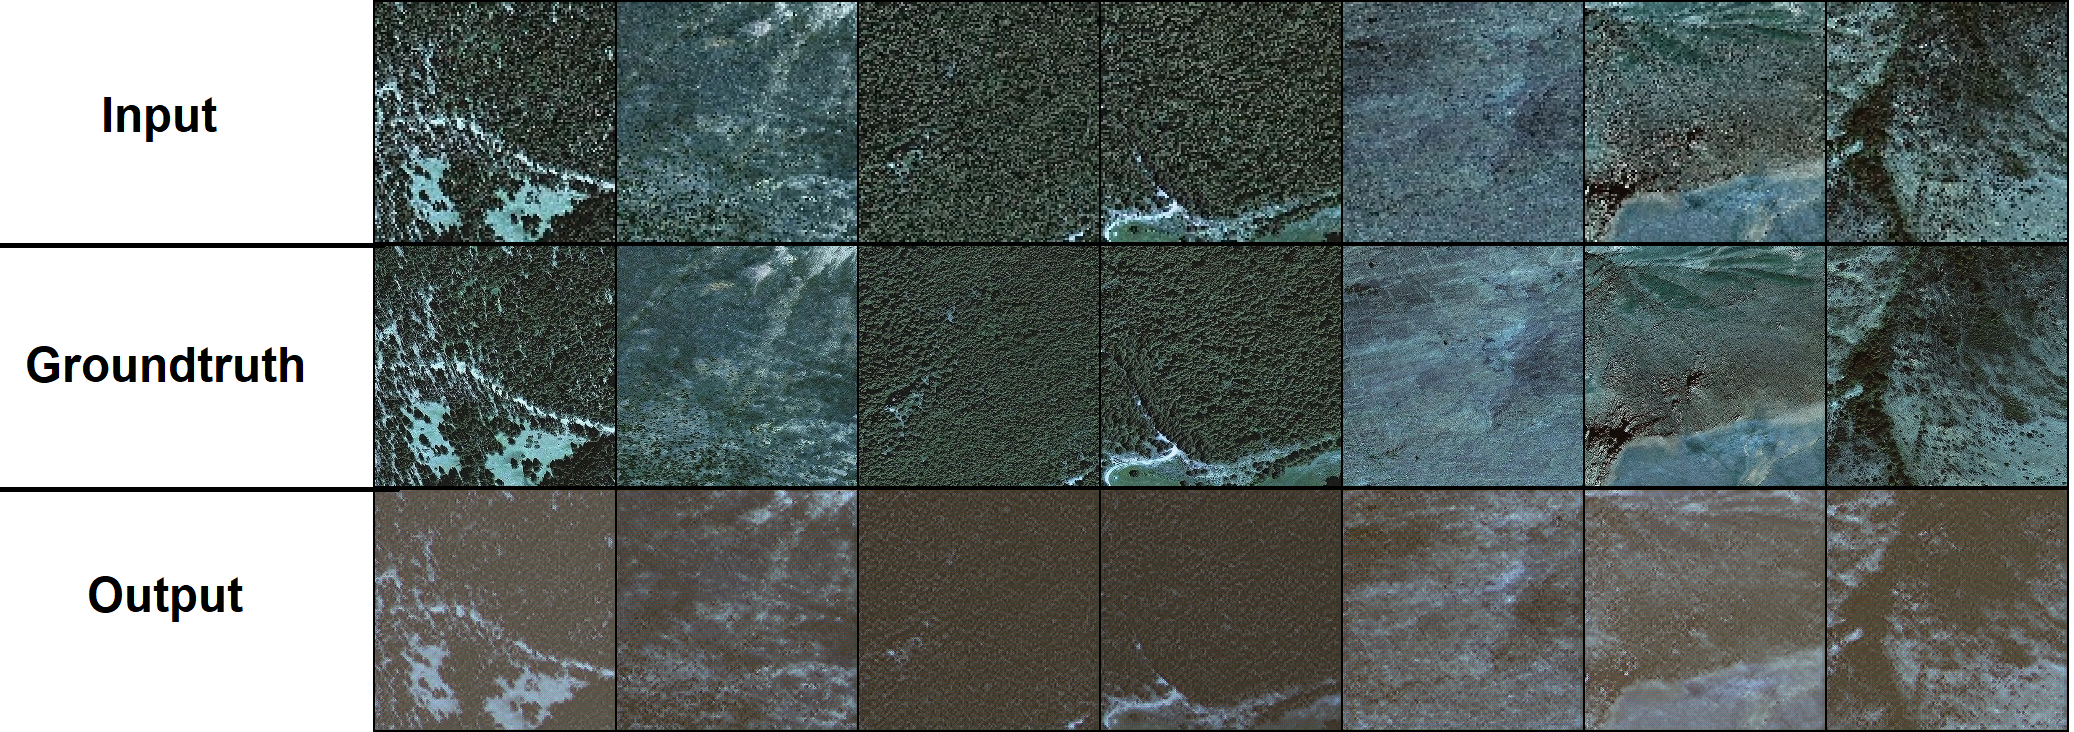
\includegraphics[width=.9\textwidth]{img/resultatGAN.png}
\caption{Resultats obtinguts amb la SRGAN}
\label{fig:resultsGAN}
\end{figure*}
\subsection{Resultats de la superresolució amb la GAN}
Per culpa del gran tamany d'aquesta xarxa, aquesta no va poder ser entrenada a Kaggle com es va fer amb la UNet, ja que aquesta plataforma només permetia executar un arxiu durant un màxim de 9 hores seguides. Per aquest motiu es va haver de migrar la xarxa a Azure, un entorn de Microsoft que ens oferia una \textit{NVIDIA Tesla K80} per 0,55€ l'hora.\\
A l'hora d'entrenar-la, vam decidir reduir la mida de les imatges i poder augmentar així el tamany dels batches, arribant a entrenar la xarxa amb un 70\% del dataset i amb batches de 15 imatges.\\ Un cop entrenada, vam aplicar les mètriques anteriors i vam obtenir els següents resultats:\\
Vam obtenir un PSNR mitjà de 60,43 dB, el qual és un valor molt més alt que el que es va obtenir amb la UNet. No obstant, si calculem el PSNR de la imatge original amb el groundtruth podem observar com aquest és de 65,08 dB, és a dir, que la nostra xarxa no ha pogut aplicar la millora desitjada a la imatge.\\
Per altra banda, si ens fixem en el SSIM podem observar com es repeteixen els resultats, obtenint un 0,17 amb les sortides de la xarxa i un 0,43 amb les imatges originals.\\

Aquest empitjorament és degut segurament a una falta d'entrenament de la xarxa, ja que aquesta estava dissenyada per ser entrenada durant més de 100 èpoques d'entrenament i durant aquest treball només se'n van poder realitzar 15.

\subsection{Resultats del visor 3D}
Per tal de poder avaluar els resultats del visor 3D, prendrem com a mètrica el temps de resposta de les imatges i el percentatge d'error que ens ofereix el nostre servidor en demanar una imatge al ICGC.\\

Per tal d'avaluar-ho s'han pres 6 mostres de la càrrega inicial de 25 imatges de la pàgina i s'han anotat els resultats a la següent taula:
\begin{table}[H]
\begin{tabular}{|c|c|c|c|c|c|c|}
\hline
\textbf{\begin{tabular}[c]{@{}c@{}}Temps de càrrega\\ (s)\end{tabular}} & 23 & 11 & 19 & 12 & 17 & 10 \\ \hline
\textbf{Nº d'imatges faltants}                                          & 0  & 1  & 0  & 0  & 0  & 2  \\ \hline
\end{tabular}
\end{table}

Com podem observar, el nostre visor triga una mitjana de 15,5 segons en iniciar, però, tal com es pot observar a la taula, com més temps porti el servidor encès, més petit serà aquest valor.\\

Per altra banda, podem observar com el visor té una mitjana de 0,5 caselles d'error per càrrega (amb 25 imatges per càrrega), no obstant aquest valor pot variar depenent de l'estabilitat de la xarxa o de l'estat del servidor del ICGC.

\section{Conclusions}
Basant-nos en els resultats obtinguts al final d'aquest treball, podem notar que, encara que finalment no s'hagin pogut assolir tots els objectius que s'havien proposat a l'inici d'aquest treball, sí que s'ha assolit l'objectiu principal que era el de crear un visor 3D que ens permetés explorar el relleu de tota l'àrea de Catalunya. Afegidament també s'han pogut crear dos models de xarxa neuronal, la primera de les quals ha millorat les imatges originals, suavitzant-les i fent més visibles petits detalls que en un principi haurien passat desapercebuts.La segona xarxa, en canvi, ha estat falta d'entrenament, el que ha causat que no donés els resultats esperats. No obstant hem pogut veure com l'estructura de les GAN és molt potent i, ja que s'entrena a ella mateixa, pot ser capaç de generar molt bons resultats.\\
Finalment, s'ha pogut demostrar que aquest tipus de tecnologia és capaç de resoldre problemes tan complexos com la millora d'imatges i que pot ser usada en el nostre dia a dia, des de la millora d'imatges aèries per a grans companyies fins a la restauració de pel·lícules antigues.
%\section{Agraïments}


\begin{thebibliography}{15}
\bibitem{kanban}
Laia Gilibets. (2020, November 11). Metodología Kanban. Retrieved November 11, 2021, from: https://www.iebschool.com/blog/metodologia-kanban-agile-scrum/

\bibitem{trello}
Trello. (2019). Retrieved November 11, 2021, from Trello.com website: https://trello.com/

\bibitem{RUNet}
Hu, X., Naiel, M., Wong, A., Lamm, M., \& Fieguth, P. (n.d.). RUNet: A Robust UNet Architecture for Image Super-Resolution.

\bibitem{DenseUNet}
Lu, Z., \& Chen, Y. (n.d.). Dense U-net for single image super-resolution with shuffle pooling layer.
‌
\bibitem{SRGAN}
Ledig, C., Theis, L., Huszár, F., Caballero, J., Cunningham, A., Acosta, A., … Shi Twitter, W. (n.d.). Photo-Realistic Single Image Super-Resolution Using a Generative Adversarial Network.

\bibitem{Sentinel}
Sentinel. (n.d.). SentinelHub API. SentinelHub API. Retrieved September 24, 2021, from https://www.sentinel-hub.com/develop/api/

\bibitem{NASA}
NASA. (n.d.). NASA Open APIs. NASA APIs. Retrieved September 24, 2021, from https://api.nasa.gov/

\bibitem{Earth}
Google. (n.d.). Google Earth Engine |. Google Developers. Retrieved September 24, 2021, from https://developers.google.com/earth-engine

\bibitem{ign}
 Instituto Geográfico Nacional. Retrieved November 14, 2021, from: https://www.ign.es/web/ign/portal/ide-area-nodo-ide-ign

\bibitem{icgc}
Institut Cartogràfic i Geològic de Catalunya. (2014). Retrieved October 2, 2021, from Icgc.cat website: https://www.icgc.cat/

\bibitem{pytorch}
PyTorch. (2021). Retrieved December 19, 2021, from Pytorch.org website: https://pytorch.org/

\bibitem {notebookKagle}
Kaggle Code. (2021). Retrieved December 19, 2021, from Kaggle.com website: https://www.kaggle.com/gerymaligne/xarxargb
‌
\bibitem{GAN}
Wikipedia Contributors. Generative adversarial network. Retrieved January 23, 2022, from website: https://en.wikipedia.org/wiki/Generative\_adversarial\_network

‌
\bibitem{Unity}
Unity Technologies. (2020). Unity - Unity. Retrieved October 9, 2021, from Unity website: https://unity.com/es

‌
\bibitem{unreal}
Unreal Engine | The most powerful real-time 3D creation tool. (2019). Retrieved October 9, 2021, from website: https://www.unrealengine.com

‌
\bibitem{godot}
Godot Engine. (2021). Free and open source 2D and 3D game engine. Retrieved October 9, 2021, from Godot Engine website: https://godotengine.org/

\bibitem{Three}
Three.js – JavaScript 3D Library. (2021). Retrieved October 9, 2021, from Threejs.org website: https://threejs.org/
‌
‌
\end{thebibliography}

\begin{comment}
\clearpage
\onecolumn
\begin{appendix}
\appendix
\section{Apèndix}

\begin{figure}[H]
\centering
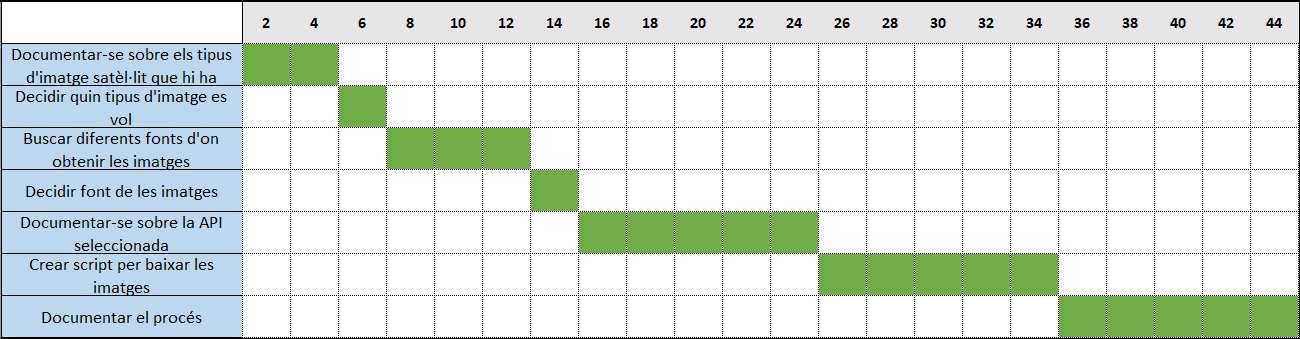
\includegraphics[width=\textwidth]{img/diagrama1.png}
\caption{Diagrama de Gantt del primer objetiu (en hores)}
\label{fig:diagrama1}
\end{figure}

 \begin{figure}[H]
\centering
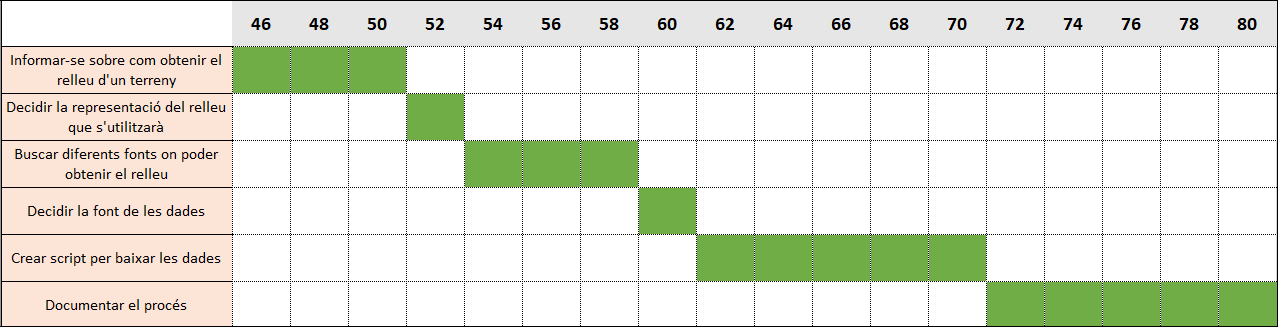
\includegraphics[width=\textwidth]{img/diagrama2.png}
\caption{Diagrama de Gantt del segon objetiu (en hores)}
\label{fig:diagrama2}
\end{figure}

\begin{figure}[H]
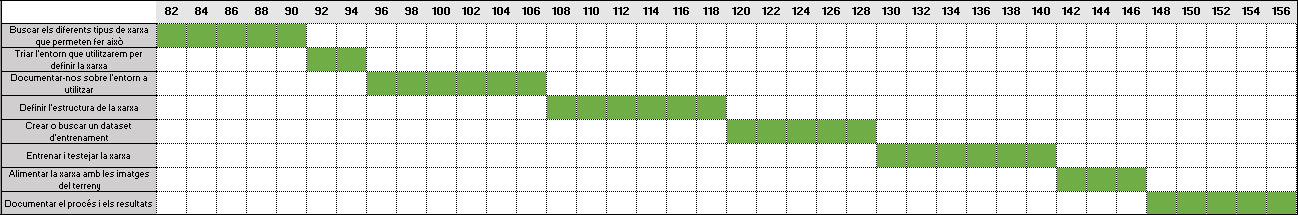
\includegraphics[width=\textwidth]{img/diagrama3.png}
\caption{Diagrama de Gantt del tercer objetiu (en hores)}
\label{fig:diagrama3}
\end{figure}

 \begin{figure}[H]
\centering
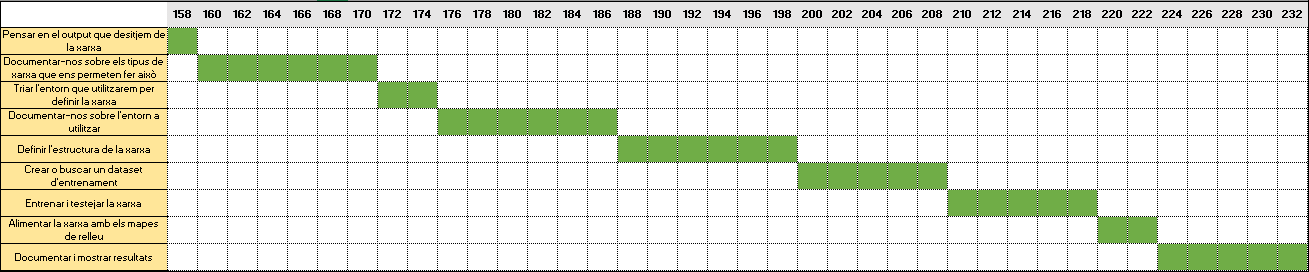
\includegraphics[width=\textwidth]{img/diagrama4.png}
\caption{Diagrama de Gantt del quart objetiu (en hores)}
\label{fig:diagrama4}
\end{figure}

 \begin{figure}[H]
\centering
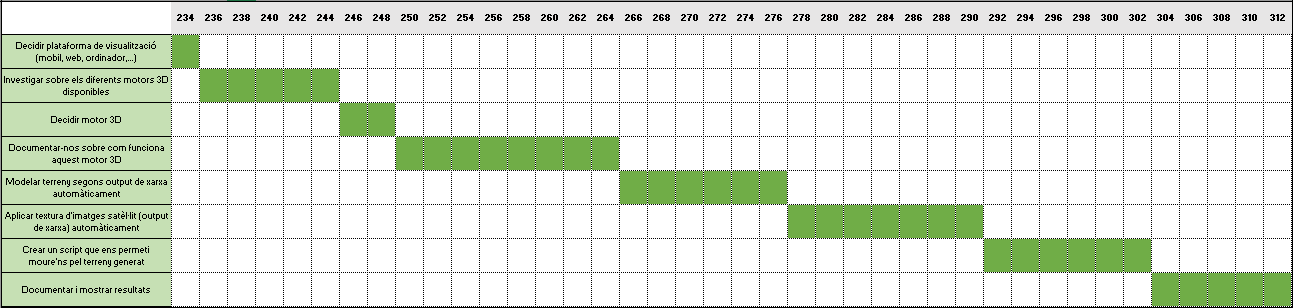
\includegraphics[width=\textwidth]{img/diagrama5.png}
\caption{Diagrama de Gantt del cinquè objetiu (en hores)}
\label{fig:diagrama5}
\end{figure}

\end{appendix}
\end{comment}
\end{document}

